\documentclass[11pt,a4paper]{article}
\usepackage[utf8]{inputenc}
\usepackage[italian]{babel}
\usepackage{amsmath}
\usepackage{amsfonts}
\usepackage{amssymb}
\usepackage{graphicx}
\usepackage{minted}
\usepackage{enumitem}
\usepackage{hyperref}
\usepackage{tikz}
\usetikzlibrary{automata, positioning, arrows}
\usepackage[left=2cm,right=2cm,top=2cm,bottom=2cm]{geometry}
\author{\Large Davide Grazzani}
\title{\Huge \Huge Progetto Reti Logiche}
\date{}
\begin{document}
    \maketitle
    \newpage

    \tableofcontents
    \newpage

    \section{Codifiche Convoluzionali e Introduzione al Progetto}
    Una codifica convoluzionale è un tipo di codifica utilizzata per la \textit{Forward Error Correction} (FEC) in sistemi di telecomunicazioni basati su canali monodirezionali. \\
    Quindi un codice generato da una codifica convoluzionale, detto anche codice convoluzionale, è un codice che trasforma ogni parola $P_1$ in una parola $P_2$. Definite $l_1 = lenght(P_1)$ e $l_2 = lenght(P_2)$ si definisce il rapoorto $l_1/l_2$ come \textit{tasso di trasmissione del convolutore} (rate); $l_2 \geq l_1$.\
    Inoltre la trasformazione è una funzione degli ultimi $k$ bit in entrata, $k$ è quindi la \textit{lunghezza dei vincoli} del codice.\\
    Lo scopo del progetto è quello di implementare un componente hardware, tramite l'utilizzo del linguaggio di specifica dello hardware VHDL, in grado di interfacciarsi con una memoria ram e di applicare una codifica convoluzionale con $rate = \frac{1}{2}$ e $k = 3$.
    \begin{figure}[h]
        \centering
        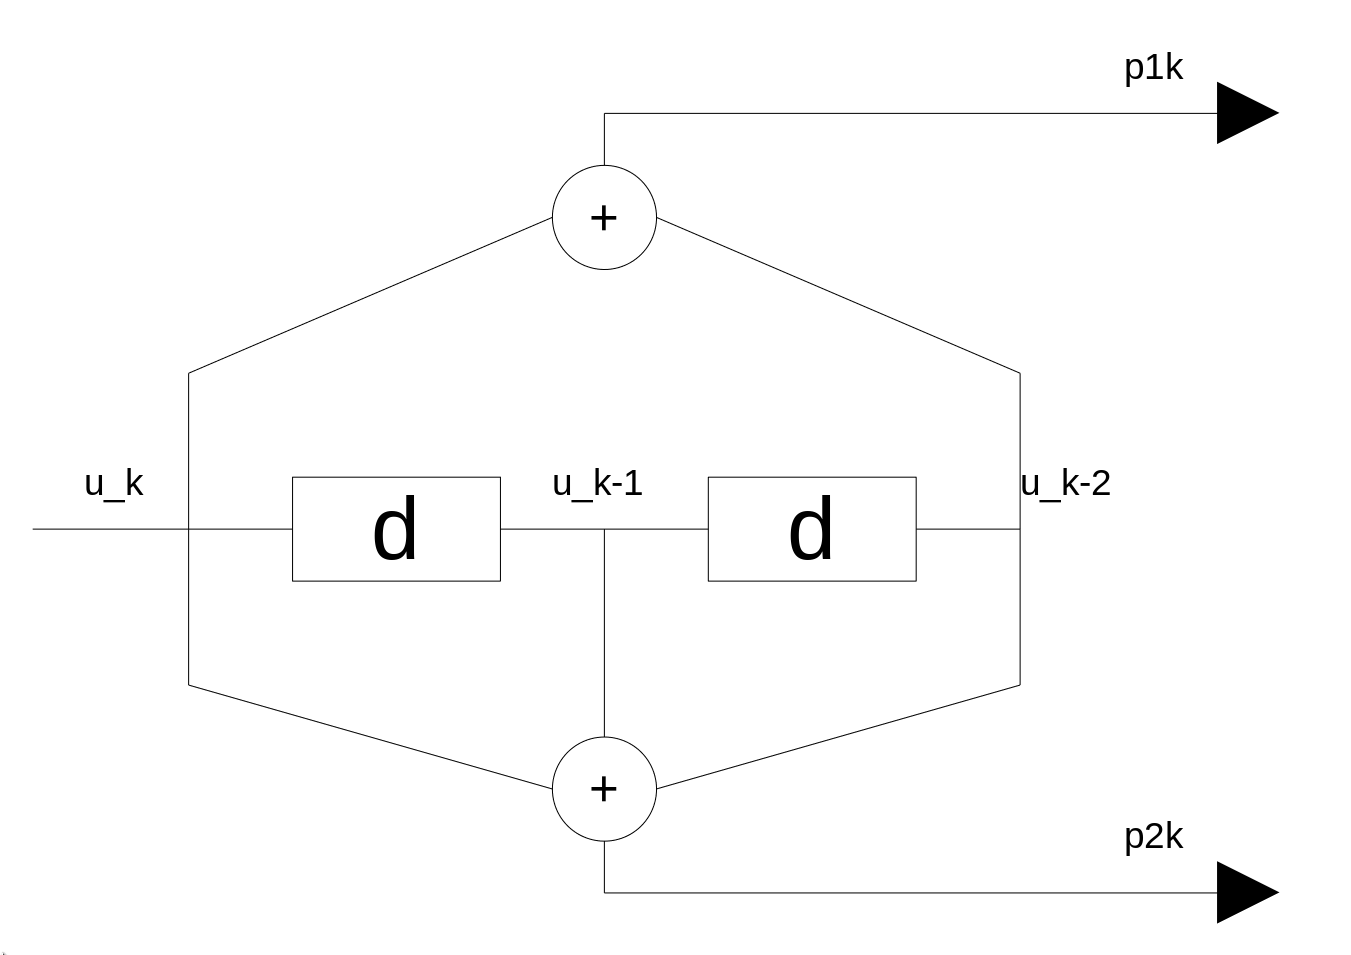
\includegraphics[width = 0.5\linewidth]{convolutore_image.png}
        \caption{Codificatore convoluzionale con $r = \frac{1}{2}$ e $k = 3$}
        \label{codificatore_convoluzionale_image}
    \end{figure}
    \subsection{Specifiche del progetto}
        Vengono fornite l'interfaccia del progetto, la specifica della memoria sulla quale interfacciarsi ed infine una limitazione temporale che impone che il modulo hardware computi correttamente con periodi di clock di almeno $clockPeriod_{req} = 100ns$.\\
        Di seguito viene riportata l'interfaccia del modulo e l'interfaccia della memoria.
        \subsubsection{Interfaccia del progetto}
            \begin{minted}{vhdl}
entity project_reti_logiche is
    port (
        i_clk : in std_logic;
        i_rst : in std_logic;
        i_start : in std_logic;
        i_data : in std_logic_vector(7 downto 0);
        o_address : out std_logic_vector(15 downto 0);
        o_done : out std_logic;
        o_en : out std_logic;
        o_we : out std_logic;
        o_data : out std_logic_vector (7 downto 0)
    );
end project_reti_logiche;
            \end{minted}
        \newpage
        \subsubsection{Interfaccia della memoria}
            \begin{minted}{vhdl}
entity rams_sp_wf is
    port(
        clk : in std_logic;
        we : in std_logic;
        en : in std_logic;
        addr : in std_logic_vector(15 downto 0);
        di : in std_logic_vector(7 downto 0);
        do : out std_logic_vector(7 downto 0)
    );
end rams_sp_wf;
            \end{minted}
            Per maggiori dettagli viene fornito il link alla \textit{User Guide} di \textit{Vivado} dalla quale la memoria è stata derivata : \url{https://www.xilinx.com/support/documentation/sw\_manuals/xilinx2017\_3/ug901-vivado-synthesis.pdf}
    \section{Architettura, approccio e scielte implementative}
        In questa sezione verrà descritta la \textit{FSM} del progetto seguita da un rapido overview sul codice presentato. Prima però vengono riportate alcune doverose considerazioni
        riguardanti il linguaggio di programmazione VHDL.
        \subsection{Considerazioni su VHDL}
            In questo progetto, durante la fase di progettazione e successivamente di sviluppo, non verrà preso mai in considerazione l'utilizzo del costrutto \textit{process} e di conseguenza
             di architetture di tipo \textit{behavioral} . Questa scelta implementativa, che si riflette sia in fase di sintesi che di implementazione, \underline{non è dovuta} al fatto che l'autore 
             del progetto creda che l'utilizzo di \textit{process} sia scorretto in qual si voglia forma o maniera; qui si vogliono riconoscere le potenzialità e le funzionalità implementative/strutturali 
             che ne derivano dall'utilizzo di quest'ultimi ma si vuole anche risaltare il maggior strato di astrazione portato da questo costrutto rispetto ad architetture \textit{dataflow} o \textit{structural} (aumento presumibilmente
             dovuto alle serializzazione di istuzioni che per natura fisica di un componente hardware dovrebbero essere paralle).\\
            È per il motivo sopra citato e per la non diretta corrispondenza tra codice scritto e struttura interna del sintetizzato hardware che in questo progetto sono state scartate implementazioni di tipo \textit{behavioral}.
        \subsection{Primo design della FSM}
            Tenendo conto delle considerazioni sopra fatte viene ora presentata la prima macchina a stati in grado già di soddisfare ampiamente requisiti di timing sia post sintesi sia post implementazione; viene discussa quest'ultima in 
            quanto alla base del design finale e da considerarsi design ottimale per periodi di clock $clockPeriod \approx [35,100] ns$.
            \newpage
            \subsubsection{Stati della macchina}
                \begin{figure}[h]
                    \centering
                    \begin{tikzpicture}[>=stealth',shorten >=1pt,auto,node distance=3cm,initial text =\texttt{Reset}]
                        \node[state, initial, initial where=left] (i)                    {$idle$};
                        \node[state]                              (r_wc) [right of=i]    {$r_{wc}$};
                        \node[state]                              (r)    [right of=r_wc] {$ r  $};
                        \node[state]                              (p_0)  [right of=r]    {$p_0 $};
                        \node[state]                              (p_1)  [right of=p_0]  {$p_1 $};
                        \node[state]                              (p_2)  [right of=p_1]  {$p_2 $};
                        \node[state]                              (p_3)  [below of=p_2]  {$p_3 $};
                        \node[state]                              (p_4)  [left of=p_3]   {$p_4 $};
                        \node[state]                              (p_5)  [left of=p_4]   {$p_5 $};
                        \node[state]                              (p_6)  [left of=p_5]   {$p_6 $};
                        \node[state]                              (p_7)  [left of=p_6]   {$p_7 $};
                        \node[state]                              (d)    [left of=p_7]   {$ d  $};
                        \path[->] (i)      edge [loop above] node {\texttt{start = '0'}} (i);
                        \path[->] (i)      edge              node {start = '1'}          (r_wc);
                        \path[->] (r_wc)   edge              node {}                     (r);
                        \path[->] (r)      edge              node {}                     (p_0);
                        \path[->] (p_0)    edge              node {}                     (p_1);
                        \path[->] (p_1)    edge              node {}                     (p_2);
                        \path[->] (p_2)    edge              node {}                     (p_3);
                        \path[->] (p_3)    edge              node {}                     (p_4);
                        \path[->] (p_4)    edge              node {}                     (p_5);
                        \path[->] (p_5)    edge              node {}                     (p_6);
                        \path[->] (p_6)    edge              node {}                     (p_7);
                        \path[->] (p_7)    edge              node {}                     (d);
                        \path[->] (d)      edge [loop below] node {$wc = 0$}             (d);
                        \path[->] (d)      edge              node {\texttt{start = '0'}} (i);
                        \path[->] (d)      edge              node {$wc \neq 0$}          (r);
                    \end{tikzpicture}
                    \caption{Primo design della \textit{FSM}}
                    \label{prima_fsm}
                \end{figure}
                con $wc$ definito come numero di parole ancora da codificare.
                \begin{description}[leftmargin = 0cm]
                    \item[Idle - $idle$ : ] stato della macchina iniziale dove questa attende che il segnale \texttt{i\_start} venga portato alto; una volta che ciò accade in questo stato vengono anche settati \texttt{o\_en = '1'} e \texttt{o\_address = 0} in modo tale da rendere il modulo pronto a ricevere il numero di parole dalla ram. Questo anche coincide con lo stato di reset della FSM.
                    \item[Read word count - $r_{wc}$ : ] stato della macchina dove viene settato il numero di parole da codificare.
                    \item[Read word - $r$ : ] stato della macchina adibito alla lettura della prossima parola da codificare. In particolare in questo stato vengono settati i valori valori di \texttt{o\_en = '1'} e \texttt{o\_address = '1'} in modo tale da leggere la parola da codificare in questo ciclo della FSM
                    \item[Process - $p_0 \rightarrow p_7$ : ] serie di 8 stati della macchina utilizzati per l'effettiva codifica della parola. Questi servono in particolare a ciclare sul singolo bit della parola considerata, oltre a contribuire alla sincronizzazione dei sottomoduli del progetto(descritto in maniera dettagliata più avanti). Espandiamo specificatamente:
                    \begin{itemize}
                        \item $p_0$ : in questo stato viene anche letta la parola richiesta precedentemente nello stato $r$.
                        \item $p_3$, $p_4$ : in questi stati vengono settati \texttt{o\_en = '1'} e \texttt{o\_we = '1'} in modo tale da poter parallelizzare la scrittura della parola in memoria con la sua effettiva computazione.
                    \end{itemize}
                    \item[Done - $d$ : ] stato della macchina che si dedica al controllo del numero di parole rimaste da codificare. Se il numero di parole è $\neq 0$ allora la FSM ritornerà alla stato $r$ altrimenti rimarrà in qiesto stato fintanto che \texttt{i\_start = '1'}.
                \end{description}
        \subsection{Design finale della FSM}
            Come precedentemente scritto la macchina sopra specificata superava i test bench per periodi di clock $clockPeriod \approx [15,100] ns$ nelle simulazione behavioral e post-sintesi ma falliva post-implementazione per $clockPeriod <\approx 35 ns$ dove le latenze dell'FPGA erano maggiori.\\
            Possibile soluzione sarebbe quella di aggiungere altri 2 stati così da poter mitigare i ritardi dovuti alla lettura della memoria. Vengono quindi qui sotto riportate delle semplici, seppur doverose, analisi in termini di tempo e di spazio per poter giustificare il cambiamento delle stuttura della macchina a stati.
            \subsubsection{Analisi di trade-off spaziale}
                Considerando il numero di stati $numStati = 12$ e utilizzando la codifica binaria $log_2(numStati) \approx 3.6$ quindi si utilizzano 4 bit per la rappresentazione di tali stati. È facile verificare che l'aggiunta di 2 stati, quindi $numStati = 14$, non richiede allocamento aggiuntivo di memoria su FPGA.
            \subsubsection{Analisi di trade-off temporale} \label{cap:tradeoff_temporale}
                Essendo uno di questi 2 stati aggiuntivi eseguito solo una volta in fase di lettura del numero di parole contenuto in ram esso verrà trascurato perchè asintoticamente irrilevante. Tenendo in considerazione gli stati che vengono eseguiti in \textit{loop}, facendo riferimento alla figura \ref{prima_fsm} gli stati da $r$ a $d$, si ottine $numStati_{m1} = 10$ e $numStati_{m2} =numStati_{m1} + 1= 11$.\\
                Quindi perchè questa modifica alla FSM sia motivata si deve avere che 
                \begin{gather*}
                    numStati_{m1} * clockPeriod_{\textit{\text{m1 min}}} > numStati_{m2} * clockPeriod_{m2} 
                \end{gather*}
                con $clockPeriod_{m1 \space min} = 35 ns$.\\
                Si ottiene che $clockPeriod_{m2} \leq 31.82 ns$, condizione che verrà poi verificata e discussa nella sezione riguardante i risultati sperimentali.
            \subsubsection{Nuova macchina a Stati}
                Vengono così aggiunti altri 2 stati :
                \begin{description}
                    \item[Wait word count - $w_{wc}$]
                    \item[Wait - $w$]  
                \end{description}
                entrambi adibiti alla mitigazione del ritardo dovuto alla lettura della memoria e alla propagazione di tale segnale in fase di implementazione.
                \begin{figure}[h]
                    \centering
                    \begin{tikzpicture}[>=stealth',shorten >=1pt,auto,node distance=3.5cm,initial text =\texttt{Reset}]
                        \node[state, initial, initial where=left] (i)                    {$idle$};
                        \node[state]                              (w_wc) [right of=i]    {$w_{wc}$};
                        \node[state]                              (r_wc) [right of=w_wc] {$r_{wc}$};
                        \node[state]                              (r)    [right of=r_wc] {$ r  $};
                        \node[state]                              (w)    [below of=r]    {$ w  $};
                        \node[state]                              (p)    [left of=w]     {$p$};
                        \node[state]                              (d)    [left of=p]     {$ d  $};
                        \path[->] (i)      edge [loop above] node {\texttt{start = '0'}} (i);
                        \path[->] (i)      edge              node {start = '1'}          (w_wc);
                        \path[->] (w_wc)   edge              node {}                     (r_wc);
                        \path[->] (r_wc)   edge              node {}                     (r);
                        \path[->] (r)      edge              node {}                     (w);
                        \path[->] (w)      edge              node {}                     (p);
                        \path[->] (p)      edge              node {}                     (d);
                        \path[->] (d)      edge [loop below] node {$wc = 0$}             (d);
                        \path[->] (d)      edge              node {\texttt{start = '0'}} (i);
                        \path[->] (d)      edge              node {$wc \neq 0$}          (r);
                    \end{tikzpicture}
                    \caption{Design finale compatto della \textit{FSM} finale}
                    \label{seconda_fsm}
                \end{figure}\\
                \textbf{Nota :} In figuara \ref{seconda_fsm} gli stati $p_0,p_1,...,p_7$ sono compressi in un unico stato $p$ al solo fine di alleggerire la notazione della macchina. Essi rimangono quindi separati come mostrato in figura \ref{prima_fsm}.
        \subsection{Code overview}
            L'obbitettivo di questa sezione è quello di mettere in relazione, e quindi eventualmente far chiarezza, le scelte implementative precedentemente introdotte con l'effettivo codice VHDL del progetto.\\
            Il progetto è composto da 3 principali componenti :
            \begin{itemize}
                \item \texttt{controller}
                \item \texttt{convolutional\_encoder}
                \item \texttt{string\_manager}
            \end{itemize}
            Successivamente vengono riportate le interfaccie dei componenti e una breve spiegazione sulle funzionalità implementate.
            \subsubsection{\texttt{controller}}
            È il responsabile per il "comportamento" del componente. Oltre ad essere responsabile per il corretto cycling degli stati, controlla direttamente i segnali di \texttt{o\_en}, \texttt{o\_we} e \texttt{o\_address}. 
                \begin{minted}{vhdl}
entity controller is
    port(
        clock            : in std_logic; --> i_clock
        reset            : in std_logic; --> i_reset
        start            : in std_logic; --> i_start
        data             : in std_logic_vector (7 downto 0); --> i_data
        done             : out std_logic := '-'; --> o_done
        mem_address      : out std_logic_vector(15 downto 0); --> o_address
        mem_enable       : out std_logic; --> o_en
        mem_write        : out std_logic; --> o_we
        u                : out std_logic; --> bit to be encoded
        component_enable : out std_logic := '0'; --> enable signal for other components
        component_reset  : out std_logic := '0' --> reset signal for other components
    );
end controller;
                \end{minted}
            \subsubsection{\texttt{convolutional\_encoder}}
                Parte del componente adibita alla codifica di un singolo bit di una parola; implementa il codificatore convoluzionale mostrato in figura \ref{codificatore_convoluzionale_image}.
                \begin{minted}{vhdl}
entity convolutional_encoder is 
    port(
        u      : in std_logic; --> u
        clock  : in std_logic; --> i_clock
        reset  : in std_logic; --> component_reset
        enable : in std_logic; --> component_enable
        pk     : out std_logic_vector(1 downto 0) --> encoder's output
    );
end convolutional_encoder;
                \end{minted}
            \subsubsection{\texttt{string\_manager}}
                Questo modulo del componente ha il compito di concatenare i 2 bit di output del \texttt{convolutional\_encoder} per formare una parola in uscita, da scrivere successivamente in memoria.
                \begin{minted}{vhdl}
entity string_manager is
    port(
    clock  : in std_logic; --> i_clock
    reset  : in std_logic; --> component_reset
    enable : in std_logic; --> component_enable
    bits   : in std_logic_vector(1 downto 0); --> pk
    half_z : out std_logic_vector(7 downto 0) --> o_data
    );
end string_manager;
                \end{minted}
            \subsubsection{Schematico del codice}
                Viene qui riportata un'immagine che mostra i collegamenti fra le varie entità del codice VHDL. La descrizione di tali collegamenti si può ritrovare nell'architettura, di tipo \textit{structural}, dell'entità \texttt{project\_reti\_logiche}.
                \begin{figure}[h]
                    \centering
                    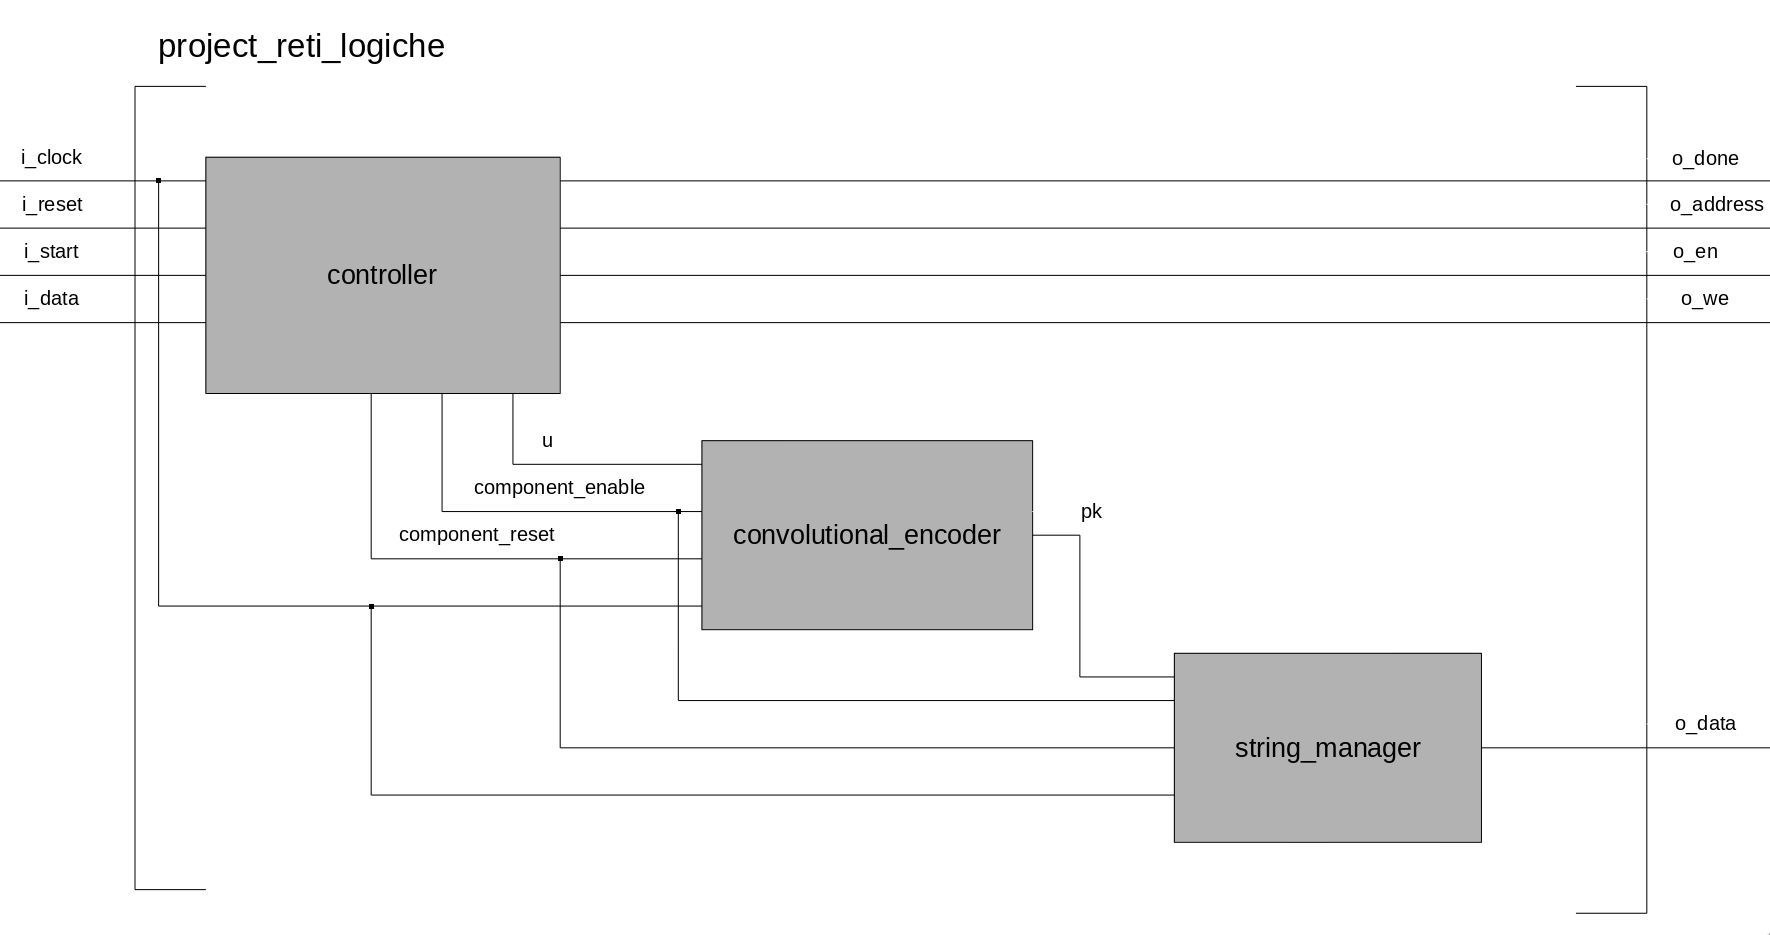
\includegraphics[width = \linewidth]{progetto_reti_logiche.png}
                    \caption{Schematico dei collegamenti tra le varie entità}
                    \label{collegamento_entità}
                \end{figure}
    \section{Risultati sperimentali}
        In questa sezione verranno discussi tutti i risultati ottenuti attraverso i vari tipi di simulazioni insieme a quali tipi di test siano stati usati per assicurare il corretto funzionamento del componente; successivamente vengono riportati alcuni dati sperimentati direttamente ottenuti dal tool di sintesi ed implementazione \textit{Vivado}.
        Vengono però prima riportate le dimensioni, in termini di \textit{LUT} e \textit{FF}, del componente hardware implementato.
        \begin{description}
            \item[LUT : ] TODO numero
            \item[FF : ] TODO numero 
        \end{description}
        \textbf{Nota :} tutti i test eseguiti sono stati eseguiti su FPGA \textit{Artix-7 xc7a200tfbg484-1}.
        \subsection{Simulazioni}
            Come precedentemente accennato le simulazioni \textit{behavioral} e quelle di \textit{Post-Synthesis} (sia \textit{Functional} che \textit{Timing}) ottenevano esiti positivi già utilizzando la FSM in figura \ref{prima_fsm} con un range di clock $clockPeriod \approx [15,100] ns$.
            Per assicurare però un minimo standard di qualità si è comunque preferito testare il componente anche in \textit{Post-Implementation}.
            È proprio dalla neccessità di ottenere un componente in grado di funzionare correttamente in  \textit{Post-Implementation} con periodi di clock $clockPeriod \approx 15 ns$ che ha portato ad una modifica della prima macchina a stati finiti ottenendo il design finale mostrato in figura \ref{seconda_fsm}.\\
            Grazie alle simulazioni è stato possibile verificare che il modulo hardware computa correttamente per periodi di clock poco inferiori a $clockPeriod = 15$, verificando così un discreto guadagno prestazionale rispetto al primo design presentato (al capitolo \ref{cap:tradeoff_temporale} vengono presentati i calcoli temporali).
            Va comunque notato che per $clockPeriod > 31.82ns$ il design ottimale rimane ancora il primo discusso.
            \newpage
            \subsubsection{Simulazione d'esempio}
                Viene ora commentata una simulazione per mostrare il funzionamento del modulo hardware :
                \begin{description}
                    \item[Tipo di simulazione : ] behavioral
                    \item[TestBench : ] \texttt{tre\_bis.vhdl}, fornita dal docente 
                    \item[Periodo di clock : ] $15ns$ 
                \end{description}
                \begin{figure}[h]
                    \centering
                    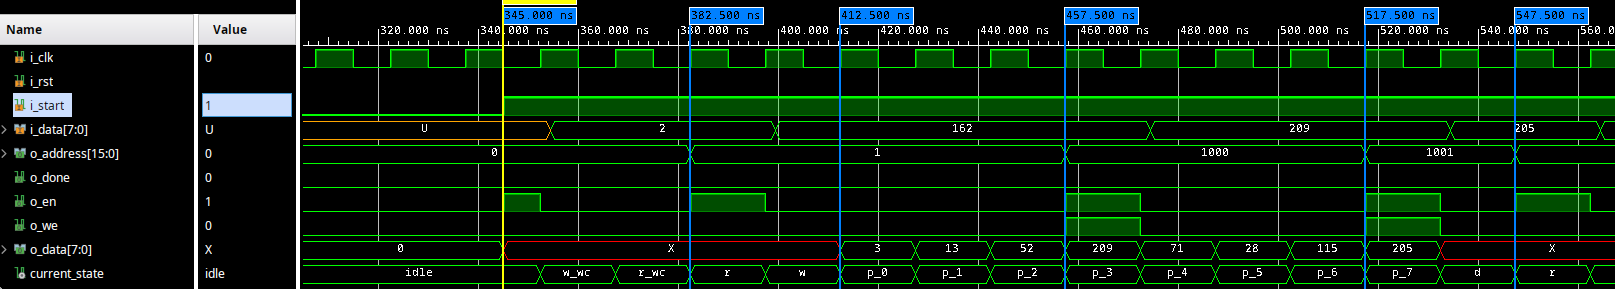
\includegraphics[width = \linewidth]{totale.png}
                    \caption{Codifica di una parola, simulazione \textit{behavioral}}
                    \label{behavioral_totale}
                \end{figure}
                La figuara \ref{behavioral_totale} mostra l'inizio della testbench e la codifica completa della parola; sulla sinistra sono presenti i sengali facenti parte dell'interfaccia del progetto insieme ad un segnale \texttt{current\_state} che rappresenta lo stato corrente della macchina.
                È stata scelta una simulazione \textit{behavioral} perchè assente da ritardi dovuti a computazione e/o propagazione, facilitandone così la lettura.\\
                Viene ora spezzata la figuara appena sopra riportata per consentirne migliore lettura.
                \begin{figure}[h]
                    \centering
                    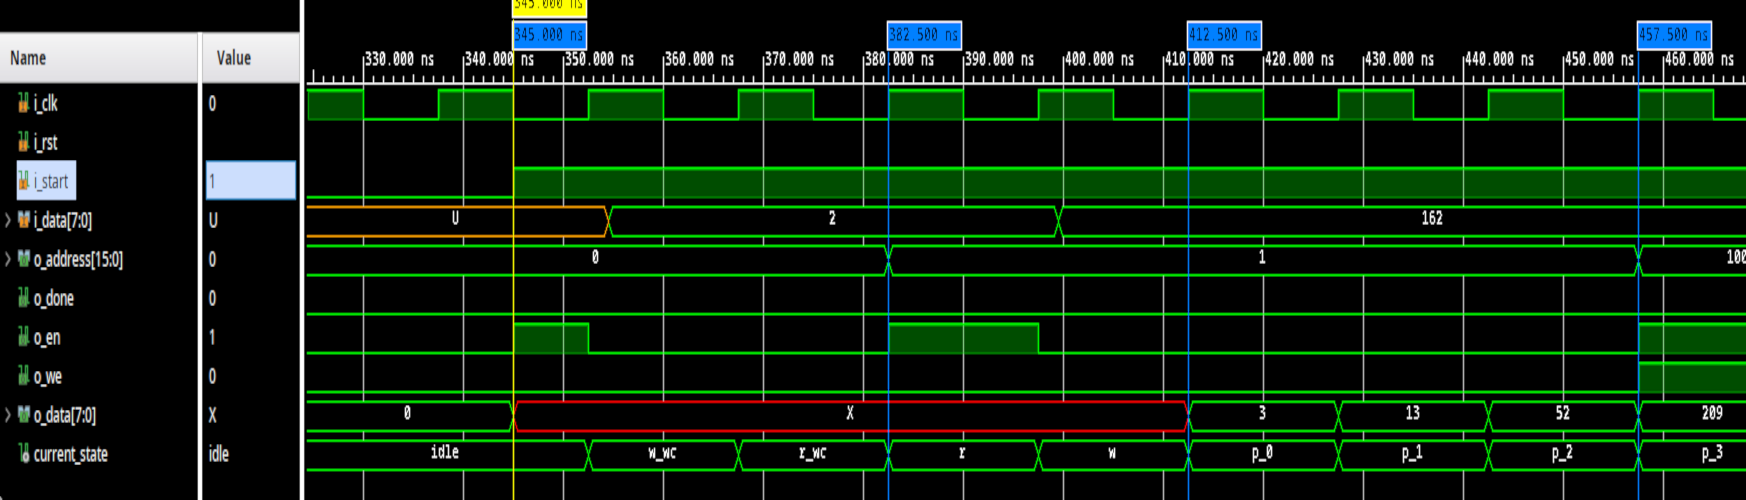
\includegraphics[width = \linewidth]{primi_4_scaled.png}
                    \caption{Inizio testbench, lettura parola, inizio computazione e scrittura prima parola codificata}
                    \label{behavioral_primi_4}
                \end{figure}
                Facendo riferimento alla figura \ref{behavioral_primi_4}
                \begin{description}[leftmargin = 0cm]
                    \item[Inizio testbench - Marker 1] La macchina si trova in stato di \textit{idle} e appena \texttt{start = '1'} viene portato \texttt{o\_en = '1'} per richiedere alla memoria il numero di parole da codificare.
                    \item[Lettura parola - Marker 2] Nella fase di \textit{read (r)} il componente porta nuovamente \texttt{o\_en = '1'} preparandosi così per la lettura di una parola.
                    \item[Inizio computazione - Marker 3] Il modulo si trova ora nella prima fase di computazione della parola \textit{$p_0$}. Viene codificato il primo bit della parola precedentemente letta e in parallelo viene aggiornato il valore di \texttt{o\_data}.
                    \item[Scrittura prima parola codifica - Marker 4] La macchina si trova nello stato \textit{$p_3$}; sta quindi codificando il quarto bit e la prima parola è già pronta per essere scritta. Si realizza così un parallelismo tra codifica e scrittura in memoria portando alto i segnali di \texttt{o\_en} e \texttt{o\_we}.
                \end{description}
                \newpage
                \begin{figure}[h]
                    \centering
                    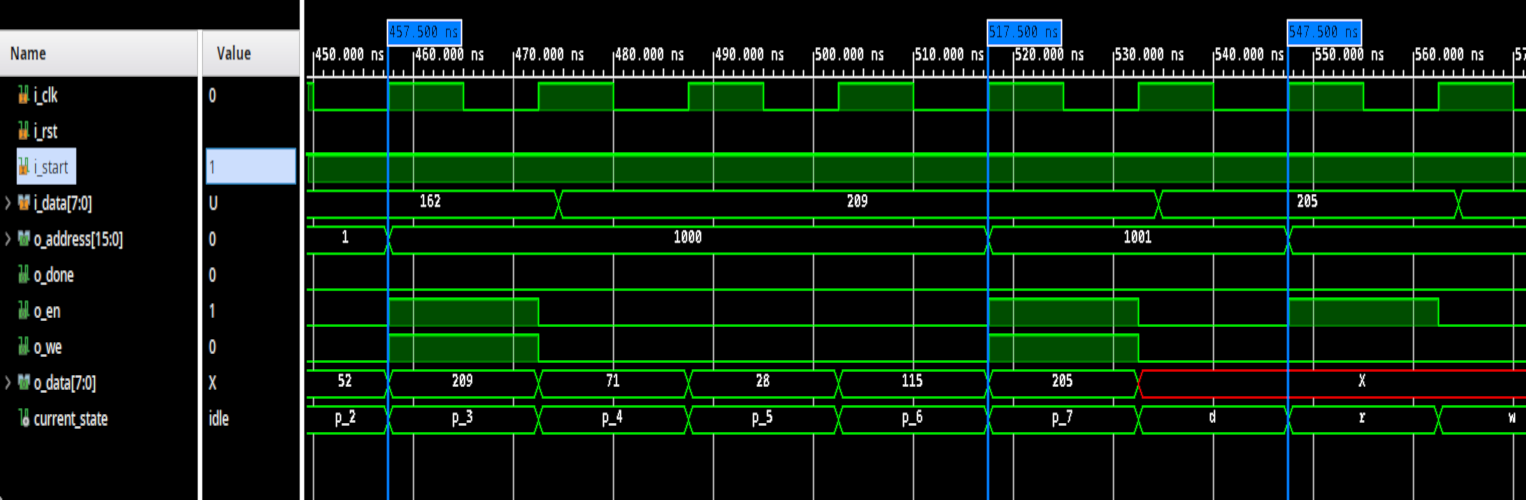
\includegraphics[width = \linewidth]{ultimi_2_scaled.png}
                    \caption{Fine codifica e lettura prossima parola}
                    \label{behavioral_ultimi_2}
                \end{figure}
                \begin{description}[leftmargin = 0cm]
                    \item[Marker 1] vedi Marker 4 in riferimento a figuara \ref{behavioral_primi_4} 
                    \item[Fine codifica - Marker 2] Nello stato \textit{$p_7$} il componente ha terminato la codifica dell'intera parola. Similmente a come accade nello stato \textit{$p_3$} (Marker 4 in riferimento a figuara \ref{behavioral_primi_4}) vi è il parallelismo tra computazione e scrittura in memoria.
                    \item[Lettura prossima parola - Marker 3] Essendo le parole da codificare 2 la FSM ritorna nello stato di \textit{read} (Marker 2).
                \end{description}
        \subsection{Testbench}
                Vengono ora qui discusse le testbench eseguite e la loro potenza di test.
                    \subsubsection{Testbench fornite dal docente} \label{cap:test_bench_docente}
                        Questa sezione di testbench comprende in particolare :
                        \begin{enumerate}
                            \item \texttt{tb\_esempio\_1.vhdl}
                            \item \texttt{tb\_esempio\_2.vhdl}
                            \item \texttt{tb\_esempio\_3.vhdl}
                            \item \texttt{tb\_seq\_max.vhdl}
                            \item \texttt{tb\_seq\_min.vhdl}
                            \item \texttt{tb\_re\_encode.vhdl}
                            \item \texttt{tb\_reset.vhdl}
                            \item \texttt{tb\_tre\_reset.vhdl}
                            \item \texttt{tb\_tre\_bis.vhdl}
                        \end{enumerate}
                        Questo set di test è molto vario così come la loro potenza.
                        \begin{description}[leftmargin = 0cm]
                            \item[Test 1, 2 e 3 : ] sono testbench iniziali per verificare il "basilare" funzionamento del componente hardware; per esempio non viene in alcun modo testata ricodifiche succesive o reset della FSM. 
                            \item[Test 4 e 5 : ] testbench utilizzate per verificare il corretto comportamento della macchina in caso di sequenze limite .
                            \item[Test 6 : ] testbench che test il re-encoding del modulo hardware (senza resettare la macchina) .
                            \item[Test 7 e 8 : ] testbench che testano le funzionalità del reset della macchina .
                            \item[Test 9 : ] testbench con $clockPeriod = 15ns$ che va ad eseguire più encoding in successione. Lo scopo di questo test è verificare il comportamento del modulo con periodi di clock molto bassi. 
                        \end{description} 
                    \subsubsection{Testbench generate attraverso tool automatico}
                        In questa sezioni vengono ulteriormente distinte :
                        \begin{itemize}
                            \item testbench generate attraverso tool automati di un collega (reperibile al seguente link : TODO link)
                            \item testbench con ram generate attraverso tool automatico (reperibile al link :TODO link   dopo la chiusura della data di consegna).\\\textit{Nota :} il tool non viene rilasciato immediatamente in quanto risedente nella stessa repository del source code del progetto stesso.
                        \end{itemize}
                        Entrambe le seguenti testbench hanno come scopo quella di verificare la correttezza del componente sintetizzato mettendo il componente stesso sotto forte stress computazionale.\\
                        Inoltre, considerando il secondo tool citato, è stato possibile riutilizzare le testbench del capitolo \ref{cap:test_bench_docente} con ram differenti aumentando così anche la loro potenza di test.
    \section{Conclusioni}
            In questo capitolo vengono discussi le limitazioni del componente sviluppato, possibili miglioramenti ed infine vengono presentati alcuni possibili campi di utilizzo del componente svilupppato. 
        \subsection{Limiti del componente hardware}
            Il modulo hardware non presenta sostanziali problematiche dall'autore rilevate. Soprattutto per $clockPeriod \approx 100ns$, definito come minimo target del progetto, il suddetto componente non presenta alcuna criticità.
            Viene invece riportato che per $clockPeriod \approx 12ns$ in simulazioni \textit{Post-Implementation, Timing} il componente non riesce a computare correttamente.
            Questo è dovuto a causa dei ritardi di computazione e di propagazione del segnale; in particolare quando il modulo vede alzare \texttt{i\_start} (fsm in stato di $idle$) non riesce a richidere alla memoria il giusto indirizzo prima del cambiamento del nuovo stato.
            Sebbene questa criticità sia nota viene scelto di non correggerla in quanto molto lontani dal minimo periodo di clock richiesto.
        \subsection{Possibili miglioramenti - Parallelismo}
            È subito immediato pensare che la migliore modifica al progetto sia quella di sfruttare le proprietà fisiche del circuito e quindi di implementare un modulo hardware in grado di codificare una parola in un solo ciclo di clock. 
            Questa modifica sarebbe possibile eliminando i flip flop che tengono in memoria gli stati precedenti del codificatore convoluzionale e collegando a cascata 8 codificatori convoluzionali modificati come precedentemente descritto.
            Il design della macchina a stati di questo componente non sarebbe diversa da quelle riportata in figura \ref{seconda_fsm}, con unica eccezione che lo stato $p$ sia effettivamente un unico stato. 
            Considerando che $numStati_{\textit{\text{m loop}}} =11$ e che $numStati_{\textit{\text{m  parallela loop}}} = 11 -7 = 4$ si ottine che :
            \begin{gather*}
                numStati_{\textit{\text{m loop}}} * 15ns > numStati_{\textit{\text{m  parallela loop}}} * clockPeriod_{\textit{\text{m  parallela}}}
            \end{gather*}
            Quindi per $clockPeriod_{\textit{\text{m  parallela}}} \leq 41.25ns$ si ottine un componente hardware più performante.\\
            Tale approccio, seppur considerato, non è stato intrapreso in quanto "snaturato" il convolutore riportato in figura \ref{codificatore_convoluzionale_image}.
        \subsection{Campi di utilizzo del modulo hardware sviluppato}
            Come già  descritto nel capitolo 1, un codificatore convoluzionale trova applicazione in sistemi di telecomunicazione dove l'integrità dell'informazione scambiata è essenziale.
            Date le dimensioni ridotte dell'implementato trova i maggiori campi d'utilizzo in dispositivi \textit{IoT} ove non è necessario l'integrazione di una \textit{Generic Purpose CPU}.
            Alcuni possibili esempi possone essere :
            \begin{itemize}
                \item telecamer
                \item dispositivi di domotica
            \end{itemize}
\end{document}